% !TeX root = surprises.tex


\chapter{The Five-Color Theorem}\label{c.five}

%%%%%%%%%%%%%%%%%%%%%%%%%%%%%%%%%%%%%%%%%%%%%%%%%%%%%%%%%%%%%%%

\abstract*{The four-color theorem states that any planar map can be colored with four colors so that no countries sharing a boundary are colored in the same color. This is a difficult theorem that was only proved in 1976. This chapter presents the relatively simple proofs of the corresponding five- and six-color theorems. The proof uses Euler's formula relating the number of vertices, edges and faces of a planar graph. Euler's formula can be used to show that two simple graphs are not planar the complete graph on five vertices and the bipartite graph with three vertices on each side are not planar.
In 1879 Alfred B. Kempe published a proof of the four-color theorem, but in 1890 Percy J. Heawood\index{Heawood, Percy J.} showed that the proof is incorrect. The chapter present Kempe's flawed proof and Heawood's demonstration that it is not correct.}

%%%%%%%%%%%%%%%%%%%%%%%%%%%%%%%%%%%%%%%%%%%%%%%%%%%%%%%%%%%%%%%

Maps use colors to distinguish one region from another by ensuring that adjacent regions are colored with different colors. In 1852 Francis Guthrie\index{Guthrie, Francis} noticed that a map of the counties of England could be colored using only four countries. The claim that four countries suffice to color any planar map is called the \emph{four-color theorem} and was only proved in 1976 by Kenneth Appel\index{Appel, Kenneth} and Wolfgang Haken\index{Haken, Wolfgang}. They used sophisticated mathematical arguments to show that if there is a counterexample (a map needing more than four colors) it had to be associated with one of $1834$ configurations. They then used a computer to check these configurations.

While the four-color theorem is extremely difficult to prove, the proofs of five- and six-color theorems stating that five or six colors are sufficient are relatively simple (Sects.~\ref{s.six-color}, ~\ref{s.five-color}). On the way to proving these theorems, we define planar maps and graphs (Sect.~\ref{s.planar}), prove Euler's formula (Sect.~\ref{s.euler}) and show that a planar graph must have vertex whose degree is less than or equal to five. In Sect.~\ref{s.nonplanar} Euler's formula is used to show that two graphs are not planar.

In 1879 Alfred B. Kempe\index{Kempe, Alfred B.} published a proof of the four-color theorem, but in 1890 Percy J. Heawood\index{Heawood, Percy J.} showed that the proof is incorrect. In Sect.~\ref{s.kempe} we present Kempe's flawed proof and Heawood's demonstration that it is not correct.

\section{Planar Maps and Graphs}\label{s.planar}

\begin{definition}
A \textit{planar map} is a set of regions in the plane separated by boundaries. A \textit{coloring} of a map is an assignment of a color to each region such that regions sharing a boundary are assigned different colors.
\end{definition}\index{Planar!map}\index{Coloring!planar graph@of a planar map}

Figure~\ref{f.five-planar-map-five} shows a five-coloring of a planar map with ten regions.
Figure~\ref{f.five-planar-map-four} shows a four-coloring of the same map.

\begin{figure}[t]
\subfigures
\leftfigure[c]{
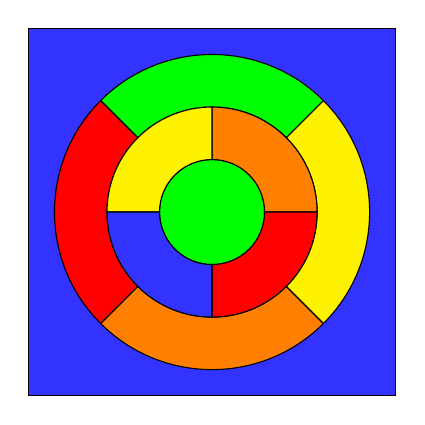
\begin{tikzpicture}[scale=.667]
\draw[fill=blue!80] (-3.5,-3.5) rectangle +(7,7);

\draw[fill=green] (0:1) 
  arc [start angle=0,  end angle=360, radius=1];

\draw[fill=green] (45:2) --
      (45:3)  arc[start angle=45,  end angle=135, radius=3] --
      (135:2) arc[start angle=135, end angle=45,  radius=2];
\draw[fill=orange] (-45:2) --
      (-45:3)  arc[start angle=-45,  end angle=-135, radius=3] --
      (-135:2) arc[start angle=-135, end angle=-45,  radius=2];
\draw[fill=yellow] (45:2) --
      (45:3)  arc[start angle=45,  end angle=-45, radius=3] --
      (-45:2) arc[start angle=-45, end angle=45,  radius=2];
\draw[fill=red] (135:2) --
      (135:3)  arc[start angle=135,  end angle=225, radius=3] --
      (225:2) arc[start angle=225, end angle=135,  radius=2];

\draw[fill=orange] (0:1) --
      (0:2)  arc[start angle=0,  end angle=90, radius=2] --
      (90:1) arc[start angle=90, end angle=0,  radius=1];
\draw[fill=red] (0:1) --
      (0:2)  arc[start angle=0,  end angle=-90, radius=2] --
      (-90:1) arc[start angle=-90, end angle=0,  radius=1];
\draw[fill=yellow] (90:1) --
      (90:2)  arc[start angle=90,  end angle=180, radius=2] --
      (180:1) arc[start angle=180, end angle=90,  radius=1];
\draw[fill=blue!80] (180:1) --
      (180:2)  arc[start angle=180,  end angle=270, radius=2] --
      (270:1) arc[start angle=270, end angle=180,  radius=1];
\end{tikzpicture}
}
\hfill
\rightfigure[c]{
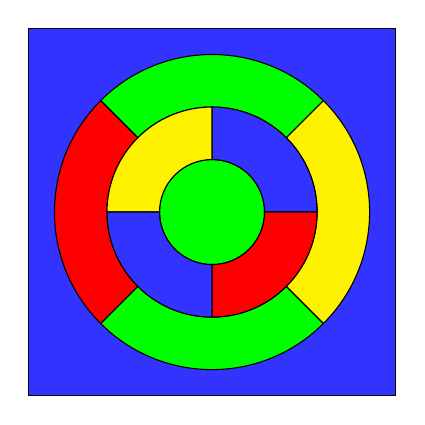
\begin{tikzpicture}[scale=.667]
\draw[fill=blue!80] (-3.5,-3.5) rectangle +(7,7);

\draw[fill=green] (0:1) 
  arc [start angle=0,  end angle=360, radius=1];

\draw[fill=green] (45:2) --
      (45:3)  arc[start angle=45,  end angle=135, radius=3] --
      (135:2) arc[start angle=135, end angle=45,  radius=2];
\draw[fill=green] (-45:2) --
      (-45:3)  arc[start angle=-45,  end angle=-135, radius=3] --
      (-135:2) arc[start angle=-135, end angle=-45,  radius=2];
\draw[fill=yellow] (45:2) --
      (45:3)  arc[start angle=45,  end angle=-45, radius=3] --
      (-45:2) arc[start angle=-45, end angle=45,  radius=2];
\draw[fill=red] (135:2) --
      (135:3)  arc[start angle=135,  end angle=225, radius=3] --
      (225:2) arc[start angle=225, end angle=135,  radius=2];

\draw[fill=blue!80] (0:1) --
      (0:2)  arc[start angle=0,  end angle=90, radius=2] --
      (90:1) arc[start angle=90, end angle=0,  radius=1];
\draw[fill=red] (0:1) --
      (0:2)  arc[start angle=0,  end angle=-90, radius=2] --
      (-90:1) arc[start angle=-90, end angle=0,  radius=1];
\draw[fill=yellow] (90:1) --
      (90:2)  arc[start angle=90,  end angle=180, radius=2] --
      (180:1) arc[start angle=180, end angle=90,  radius=1];
\draw[fill=blue!80] (180:1) --
      (180:2)  arc[start angle=180,  end angle=270, radius=2] --
      (270:1) arc[start angle=270, end angle=180,  radius=1];
\end{tikzpicture}
}
\leftcaption{Five-coloring of a planar map}\label{f.five-planar-map-five}
\rightcaption{Four-coloring of a planar map}\label{f.five-planar-map-four}
\end{figure}

\begin{definition}
A \emph{graph} is a set of \emph{vertices} $V$ and a set of \emph{edges} $E$, such that each edge is incident with exactly two vertices.

A \emph{planar graph} is a graph such that no edges cross each other. In a planar graph, areas enclosed by a set of edges are called \emph{faces}.

A \emph{coloring} of a planar graph is an assignment of colors to vertices such that no two vertices of the same color are connected by an edge.
\end{definition}\index{Planar!graph}\index{Coloring!planar graph@of a planar graph}

Planar maps and planar graphs are dual and it is convenient to investigate coloring problems in graphs rather than maps.

\begin{theorem}
Given a planar map, a planar graph can be constructed such for each coloring of the regions of the map, there is a coloring of the vertices of the graph, and conversely.
\end{theorem}

\begin{proof}
Construct one vertex for each region and construct an edge between two vertices if and only if the corresponding regions share a boundary. 
\end{proof}

\begin{example}
Figure~\ref{f.five-planar-graph-map} shows the planar map from Fig.~\ref{f.five-planar-map-four} and the vertices associated with the regions. Figure~\ref{f.five-planar-graph-graph} shows the planar graph that corresponds to the map.
\end{example}

\begin{figure}[t]
\subfigures
\leftfigure[c]{
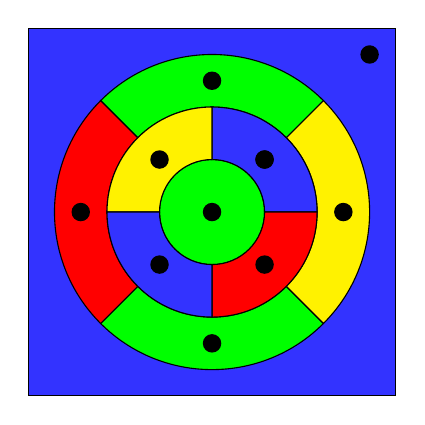
\begin{tikzpicture}[scale=.667]

\draw[fill=blue!80] (-3.5,-3.5) rectangle +(7,7);

\draw[fill=green] (0:1) 
  arc [start angle=0,  end angle=360, radius=1];

\draw[fill=green] (45:2) --
      (45:3)  arc[start angle=45,  end angle=135, radius=3] --
      (135:2) arc[start angle=135, end angle=45,  radius=2];
\draw[fill=green] (-45:2) --
      (-45:3)  arc[start angle=-45,  end angle=-135, radius=3] --
      (-135:2) arc[start angle=-135, end angle=-45,  radius=2];
\draw[fill=yellow] (45:2) --
      (45:3)  arc[start angle=45,  end angle=-45, radius=3] --
      (-45:2) arc[start angle=-45, end angle=45,  radius=2];
\draw[fill=red] (135:2) --
      (135:3)  arc[start angle=135,  end angle=225, radius=3] --
      (225:2) arc[start angle=225, end angle=135,  radius=2];

\draw[fill=blue!80] (0:1) --
      (0:2)  arc[start angle=0,  end angle=90, radius=2] --
      (90:1) arc[start angle=90, end angle=0,  radius=1];
\draw[fill=red] (0:1) --
      (0:2)  arc[start angle=0,  end angle=-90, radius=2] --
      (-90:1) arc[start angle=-90, end angle=0,  radius=1];
\draw[fill=yellow] (90:1) --
      (90:2)  arc[start angle=90,  end angle=180, radius=2] --
      (180:1) arc[start angle=180, end angle=90,  radius=1];
\draw[fill=blue!80] (180:1) --
      (180:2)  arc[start angle=180,  end angle=270, radius=2] --
      (270:1) arc[start angle=270, end angle=180,  radius=1];


\foreach \x/\y/\name in {
    0/0/O,
    3/3/Z,
    1/1/E,-1/1/F,-1/-1/G,1/-1/H,
    0/2.5/A,2.5/0/B,0/-2.5/C,-2.5/0/D,
    } {
  \fill (\x,\y) coordinate(\name) circle(5pt);
}
\end{tikzpicture}
}
\hfill
\rightfigure[c]{
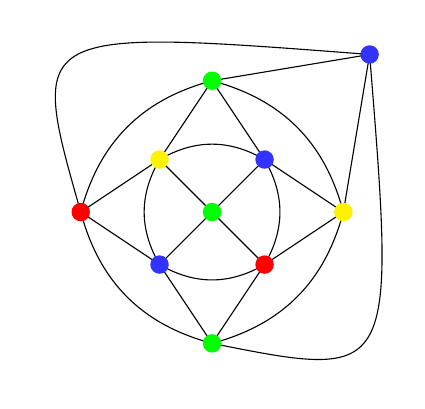
\begin{tikzpicture}[scale=.667]

\foreach \x/\y/\name in {
    0/0/O,
    3/3/Z,
    1/1/E,-1/1/F,-1/-1/G,1/-1/H,
    0/2.5/A,2.5/0/B,0/-2.5/C,-2.5/0/D,
    } {
  \coordinate(\name) at (\x,\y);
}

\draw (E) -- (O) -- (F);
\draw (G) -- (O) -- (H);
\draw (E) to [bend right=30] (F) to [bend right=30] (G) 
          to [bend right=30] (H) to [bend right=30] (E);
\draw (A) -- (E) -- (B) -- (H) -- (C) -- (G) -- (D) -- (F);
\draw (A) to [bend right=30] (D) to [bend right=30] (C) 
          to [bend right=30] (B) to [bend right=30] (A);

\draw (F) -- (A) -- (Z) -- (B);
\draw (C) .. controls (3.5,-3.2) .. (Z);
\draw (D) .. controls (-3.5,3.5) .. (Z);

\foreach \cl/\x/\y in {
    green/0cm/0cm,
    blue!80/3cm/3cm,
    blue!80/1cm/1cm,
    yellow/-1cm/1cm,
    blue!80/-1cm/-1cm,
    red/1cm/-1cm,
    green/0cm/2.5cm,
    yellow/2.5cm/0cm,
    green/0cm/-2.5cm,
    red/-2.5cm/0cm
    }
 \fill[\cl] (\x,\y) circle (5pt);
\end{tikzpicture}
}
\leftcaption{Associating vertices with the regions of a planar map}\label{f.five-planar-graph-map}
\rightcaption{The planar graph that corresponds to the planar map}\label{f.five-planar-graph-graph}
\end{figure}

We can further limit our graphs to those whose faces are triangular.

\begin{definition}
A graph is \emph{triangular} if all its faces are bounded by three edges. A graph can be \emph{triangulated} if edges can be added so that the graph is triangular. We also say that there is a \emph{triangulation} of the graph.
\end{definition}\index{Triangulated graph}

\begin{example}
The faces in the planar graph in Fig.~\ref{f.five-planar-graph-graph} are triangular since each one is bounded by three edges. The edges are curved so the faces are not triangles, which are polygons whose three edges are straight line segments.
\end{example}

\begin{advanced}
\textbf{F\'{a}ry's Theorem}\index{Fary's theorem@F\'{a}ry's theorem} states that any triangular planar graph can be be transformed into an equivalent planar graph whose edges are straight line segments. Therefore, with no loss of generality,  proofs can be restricted to  planar graphs whose faces are triangles.
\end{advanced}

\begin{example}
Fig.~\ref{f.five-triangular-graph} (left) shows that a square can be two-colored, but if it is triangulated (center), four colors are necessary. Our goal is to prove that \emph{all} graphs can be $n$-colored for some $n$. If the triangulated graph is $n$-colored, so is the original graph, because deleting the extra edges does not invalidate the coloring (right).
\end{example}

\begin{figure}[h]
\begin{center}
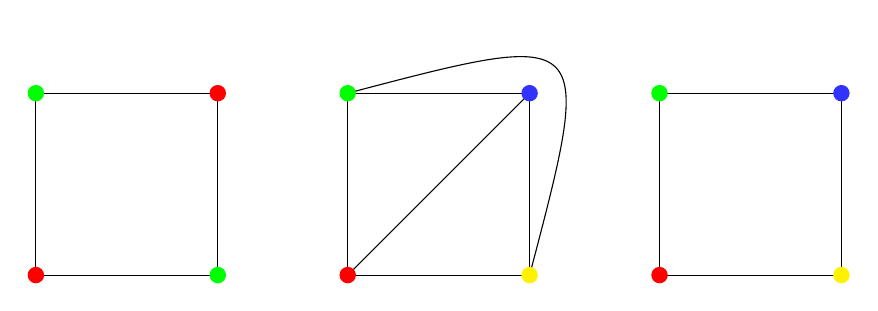
\begin{tikzpicture}[scale=.33]
\draw (-3.5,-3.5) rectangle +(7,7);
\fill[red] (-3.5,-3.5) circle(9pt);
\fill[green] (-3.5,3.5) circle(9pt);
\fill[green] (3.5,-3.5) circle(9pt);
\fill[red] (3.5,3.5) circle(9pt);
\begin{scope}[xshift=12cm]
\draw (-3.5,-3.5) -- (3.5,3.5);
\draw (-3.5,3.5) .. controls (6,6) .. (3.5,-3.5);
\draw (-3.5,-3.5) rectangle +(7,7);
\fill[red] (-3.5,-3.5) circle(9pt);
\fill[green] (-3.5,3.5) circle(9pt);
\fill[yellow] (3.5,-3.5) circle(9pt);
\fill[blue!80] (3.5,3.5) circle(9pt);
\end{scope}
\begin{scope}[xshift=24cm]
\draw (-3.5,-3.5) rectangle +(7,7);
\fill[red] (-3.5,-3.5) circle(9pt);
\fill[green] (-3.5,3.5) circle(9pt);
\fill[yellow] (3.5,-3.5) circle(9pt);
\fill[blue!80] (3.5,3.5) circle(9pt);
\end{scope}
\end{tikzpicture}
\end{center}
\caption{Coloring a triangulated graph}\label{f.five-triangular-graph}
\end{figure}

\section{Euler's Formula}\label{s.euler}

\begin{theorem}\label{thm.euler} Let $G$ be a connected planar graph with $V$ vertices, $E$ edges and $F$ faces. Then $V-E+F=2$.
\end{theorem}\index{Euler's formula}

\begin{proof}
By induction on the number of edges. If the number of edges in the connected planar graph is zero, there is only a single vertex and a single face, so $1-0+1=2$.

Otherwise, there is at least one edge $e$ and it connects two vertices $v_1,v_2$. Delete edge $e$.

\textit{Case 1:}
The graph becomes disconnected (Fig.~\ref{f.five-disconnected-removing}). Merge $v_1$ with $v_2$ (Fig.~\ref{f.five-disconnected-merge}). The resulting graph $G'$ is a planar connected graph and has fewer edges than $G$, so by the induction hypothesis, $(V-1)-(E-1)+F=2$ since the number of vertices is also reduced by one. Simplifying, we get $V-E+F=2$ for $G$.
\begin{figure}[ht]
\subfigures
\leftfigure[c]{
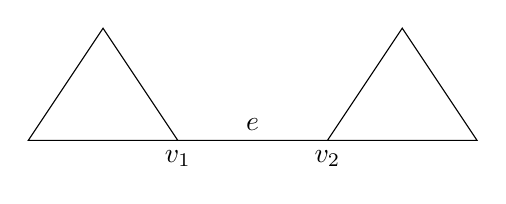
\begin{tikzpicture}[scale=.95]
\draw (2,0) -- (1,1.5) -- (0,0) -- (2,0) node[below] {$v_1$} -- node[above] {$e$} (4,0) node[below] {$v_2$} -- (6,0) -- (5,1.5) -- (4,0);
\end{tikzpicture}
}
\hfill
\rightfigure[c]{
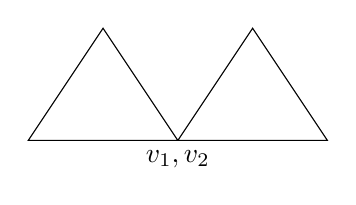
\begin{tikzpicture}[scale=.95]
\draw (2,0) -- (1,1.5) -- (0,0) -- (2,0) node[below] {$v_1,v_2$} -- (4,0) -- (3,1.5) -- (2,0);
\end{tikzpicture}
}
\leftcaption{Removing an edge disconnects the graph}\label{f.five-disconnected-removing}
\rightcaption{Merging two vertices}\label{f.five-disconnected-merge}
\end{figure}

\textit{Case 2:}
The graph remains connected (Fig.~\ref{f.five-connected-remains}). $G'$ has fewer edges than $G$ (Fig.~\ref{f.five-connected-fewer}), so by the induction hypothesis, $V-(E-1)+(F-1)=2$ since removing the edge joins two faces into one. Simplifying, we get $V-E+F=2$ for $G$.
\end{proof}

\begin{figure}[ht]
\subfigures
\leftfigure[c]{
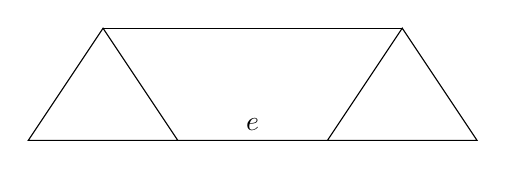
\begin{tikzpicture}[scale=.95]
\draw (2,0) -- (1,1.5) -- (0,0) -- (2,0) -- node[above] {$e$} (4,0) -- (6,0) -- (5,1.5) -- (4,0);
\draw (1,1.5) -- (5,1.5);
\end{tikzpicture}
}
\hfill
\rightfigure[c]{
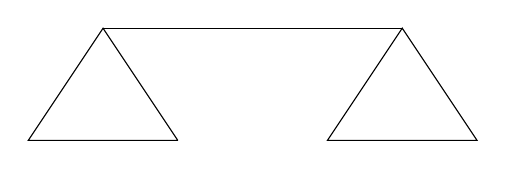
\begin{tikzpicture}[scale=.95]
\draw (2,0) -- (1,1.5) -- (0,0) -- (2,0);
\draw (4,0) -- (5,1.5) -- (6,0) -- cycle;
\draw (1,1.5) -- (5,1.5);
\end{tikzpicture}
}
\leftcaption{Removing an edge does not disconnect the graph}\label{f.five-connected-remains}
\rightcaption{The graph remains connected and has fewer edges}\label{f.five-connected-fewer}
\end{figure}


\begin{theorem}
Let $G$ be a connected, triangulated planar graph with $E$ edges and $V$ vertices. Then $E= 3V-6$.
\end{theorem}
\begin{proof}
Each face is bounded by three edges, so $E=3F/2$, where we divided by $2$ because each edge has been counted twice, once for each face it bounds. By Euler's formula:
\begin{eqnarray*}
E&=&V+F-2\\
&=&V+2E/3-2\\
&=&3V-6\,.
\end{eqnarray*}
\end{proof}

\begin{example}
The planar graph in Fig.~\ref{f.five-planar-graph-graph} has $10$ vertices and $3\cdot 10-6=24$ edges.
\end{example}

\begin{theorem}\label{thm.count}
Let $G$ be a connected planar graph. Then $E\leq 3V-6$.
\end{theorem}

\begin{proof}
Triangulate $G$ to obtain $G'$. $E'= 3V'-6$ by Thm.~\ref{thm.count}. Now remove edges from $G'$ to obtain $G$. The number of vertices does not change so  $E\leq 3V-6$.
\end{proof}

\begin{example}
The graph in Fig.~\ref{f.five-fewer} has $8$ edges and $6$ vertices, and $8< 3\cdot 6 - 6= 12$.
Figure~\ref{f.five-upper-limit} shows a triangulated graph with $6$ vertices and $3\cdot 6 - 6= 12$ edges.
\end{example}

\begin{figure}[t]
\subfigures
\leftfigure[c]{
\begin{tikzpicture}[scale=.9]
\draw (2,0) -- (1,1.5) -- (0,0) -- (2,0) -- (4,0) -- (6,0) -- (5,1.5) -- (4,0);
\draw (1,1.5) -- (5,1.5);
\path (2,0) .. controls (-1,-1) and (-1,1) .. (1,1.5);
\path (2,0) .. controls (3,-1) .. (6,0) .. controls (7,2) and (4,2) .. (1,1.5);
\end{tikzpicture}
}
\hfill
\rightfigure[c]{
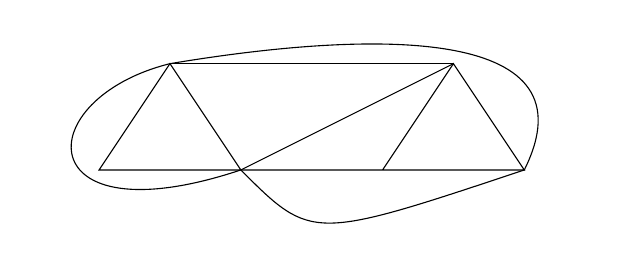
\begin{tikzpicture}[scale=.9]
\draw (2,0) -- (1,1.5) -- (0,0) -- (2,0) -- (4,0) -- (6,0) -- (5,1.5) -- (4,0);
\draw (1,1.5) -- (5,1.5);
\draw (2,0) -- (5,1.5);
\draw (2,0) .. controls (-1,-1) and (-1,1) .. (1,1.5);
\draw (2,0) .. controls (3,-1) .. (6,0) .. controls (7,2) and (4,2) .. (1,1.5);
\end{tikzpicture}
}
\leftcaption{Fewer edges than the upper limit}\label{f.five-fewer}
\rightcaption{In a triangulated graph the number of edges is maximal}\label{f.five-upper-limit}
\end{figure}

\section{Non-planar Graphs}\label{s.nonplanar}

Let us take a short detour to show how Thms.~\ref{thm.euler} and~\ref{thm.count} can be used to prove that certain graphs are not planar.

\begin{theorem}
$K_5$, the complete graph on five vertices, is not planar (Fig.~\ref{f.five-k5}).
\end{theorem}\index{K5@$K_{5}$ is not planar}

\begin{figure}[t]
\subfigures
\leftfigure[c]{
\begin{tikzpicture}[scale=.8]
\node (pentagon) [minimum size=4cm,regular polygon,regular polygon sides=5] at (0,0) {};
\draw (pentagon.corner 1) -- (pentagon.corner 2);
\draw (pentagon.corner 2) -- (pentagon.corner 3);
\draw (pentagon.corner 3) -- (pentagon.corner 4);
\draw (pentagon.corner 4) -- (pentagon.corner 5);
\draw (pentagon.corner 5) -- (pentagon.corner 1);
\draw (pentagon.corner 1) -- (pentagon.corner 3);
\draw (pentagon.corner 1) -- (pentagon.corner 4);
\draw (pentagon.corner 2) -- (pentagon.corner 4);
\draw (pentagon.corner 2) -- (pentagon.corner 5);
\draw (pentagon.corner 3) -- (pentagon.corner 5);
\end{tikzpicture}
}
\hfill
\rightfigure[c]{
\begin{tikzpicture}[scale=.8]
\node (pentagon) [minimum size=4cm,regular polygon,regular polygon sides=5] at (0,0) {};
\draw (pentagon.corner 1) -- (pentagon.corner 2);
\draw (pentagon.corner 2) -- (pentagon.corner 3);
\draw (pentagon.corner 3) -- (pentagon.corner 4);
\draw (pentagon.corner 4) -- (pentagon.corner 5);
\draw (pentagon.corner 5) -- (pentagon.corner 1);
\draw (pentagon.corner 1) .. controls (-4,1) .. 
      (pentagon.corner 3);
\draw (pentagon.corner 1) .. controls (4,1) ..
      (pentagon.corner 4);
\draw (pentagon.corner 2) -- (pentagon.corner 4);
\draw (pentagon.corner 2) -- (pentagon.corner 5);
\draw (pentagon.corner 3) -- (pentagon.corner 5);
\draw[thick] (0,-.95) circle(5pt);
\end{tikzpicture}
}
\leftcaption{$K_5$ is not planar}\label{f.five-k5}
\rightcaption{A failed attempt to draw $K_5$ as planar}\label{f.five-k5-failed}
\end{figure}

\begin{proof}
For $K_5$, $V=5$ and $E=10$. By Thm.~\ref{thm.count} the number of edges must be less than or equal to $3\cdot 5 -6=9$ so the graph is not planar.
\end{proof}

\begin{theorem}
$K_{3,3}$, the bipartite graph with three vertices on each side, is not planar (Fig.~\ref{f.five-k33}).
\end{theorem}\index{K33@$K_{3,3}$ is not planar}

\begin{figure}[b]
\subfigures
\leftfigure[c]{
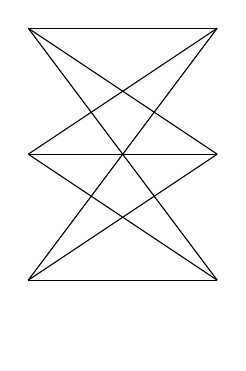
\begin{tikzpicture}[scale=.8]
\draw (0,0) -- (3,0);
\draw (0,2) -- (3,2);
\draw (0,4) -- (3,4);
\draw (0,0) -- (3,2);
\draw (0,2) -- (3,4);
\draw (0,4) -- (3,0);
\draw (0,0) -- (3,4);
\draw (0,2) -- (3,0);
\draw (0,4) -- (3,2);
\path (0,-1) -- (3,-1);
\end{tikzpicture}
}
\hfill
\rightfigure[c]{
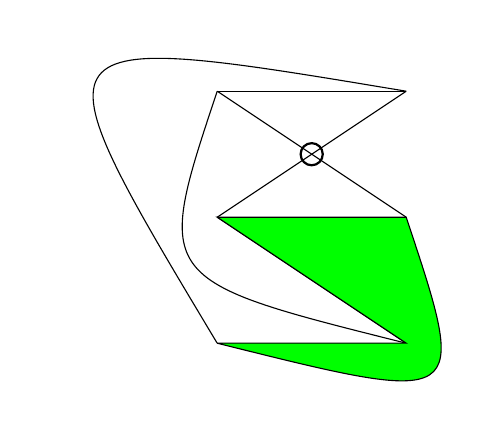
\begin{tikzpicture}[scale=.8]
\draw (0,4) -- (3,4);
\draw (0,2) -- (3,4);
\draw (0,4) .. controls (-1,1) .. (3,0);
\draw (0,0) .. controls (-3,5) .. (3,4);
\draw (0,2) -- (3,0);
\draw (0,4) -- (3,2);

\draw[fill=green] (0,0) -- (3,0) -- (3,0) -- (0,2)  -- (3,2) .. controls (4,-1) .. (0,0);
\draw[thick] (1.5,3) circle(5pt);
\end{tikzpicture}
}
\leftcaption{$K_{3,3}$ is not planar}\label{f.five-k33}
\rightcaption{A failed attempt to draw $K_{3,3}$ as planar}\label{f.five-k33-failed}
\end{figure}

\begin{proof}
$V=6$ and $E=9$. By Thm~\ref{thm.euler} if $K_{3,3}$ is planar, $F=E-V+2=9-6+2=5$. But each face is bounded by four edges (Fig.~\ref{f.five-k33-failed}), so $E=4F/2=10\neq 9$.
\end{proof}

In 1930 Kazimierz Kuratowski\index{Kuratowski Kazimierz} proved a converse to these theorems: if a graph is not planar it contains (in a certain sense) $K_5$ or $K_{3,3}$.

\section{The Degrees of the Vertices}\label{s.degrees}

\begin{definition}
$d(v)$, the \emph{degree} of vertex $v$, is the number of edges incident with $v$.
\end{definition}\index{Degree of a vertex}

\begin{example}
The graph in Fig.~\ref{f.five-planar-graph-graph} contains $8$ vertices corresponding to the two rings, each of degree $5$. The vertex corresponding to the outer face is of degree $4$ as is the vertex corresponding to the inner face. Therefore:
\[
\sum_{v\in V} d(v) = 5\cdot 8 + 4\cdot 2=48\,.
\]
To get the total number of edges divide $48$ by $2$ because  each edge was counted twice, once for each of the vertices it is incident to.
\end{example}

\newpage

By generalizing the argument we get:
\begin{theorem}\label{thm.degrees}
Let $d_i$ for $i=1,2,3,\ldots,k$, be the number of vertices of degree $i$ in a connected planar graph $G$ with $V$ vertices and $E$ edges, where $k$ is the highest degree of a vertex in $V$. Then:
\[
\sum_{v\in V} d(v) =\sum_{i=1}^{k} i\cdot d_i=2E\,.
\]
\end{theorem}

\begin{theorem}\label{thm.degree5}
Let $G$ be a connected planar graph with $E$ edges and $V$ vertices, and let $d_i$ for $i=1,\ldots,k$, be the number of vertices of degree $i$, where $k$ is the highest degree of a vertex in $V$. Then there must be a vertex $v$ in $V$ such that $d(v) \leq 5$.
\end{theorem}

\begin{proof}[1]
If there are $d_1$ vertices of degree $1$, $d_2$ vertices of degree $2$, \ldots, $d_k$ vertices of degree $k$, then $V=\sum_{i=1}^{k}d_i$.  From Thms.~\ref{thm.count} and \ref{thm.degrees}:
\[
\sum_{i=1}^{k} i\cdot d_i=2E\leq 2(3V-6) = 6V-12=6\sum_{i=1}^{k} d_i -12\,.
\]
Therefore:
%
\begin{eqnarray*}
\sum_{i=1}^{k} i\cdot d_i &\leq& 6\sum_{i=1}^{k} d_i -12\\
\sum_{i=1}^{k} (6-i)d_i&\geq& 12\,.
\end{eqnarray*}
Since $12>0$ and all $d_i$ are positive, for least one $i$, $6-i>0$ and for that $i$, $i<6$.
\end{proof}

\begin{proof}[2]
Let us compute the \emph{average} degree of the vertices, which is the sum of the degrees divided by the number of vertices:
\[
d_{\textit{\footnotesize avg}}=\frac{\sum_{i=1}^{k} i\cdot d_i}{V}\,.
\]
But the sum of the degrees is twice the number of edges which by Thm.~\ref{thm.count} gives:
\[
d_{\textit{\footnotesize avg}}=\frac{2E}{V}\leq \frac{6V-12}{V}=6-\frac{6}{V}<6\,.
\]
If the average is less than six there must be a vertex of degree less than six.
\end{proof}

\begin{example}
In Fig.~\ref{f.five-planar-graph-graph}, the sum of the degrees is $8\cdot 5 + 2\cdot 4=48$. There are $10$ vertices, so the average degree is $48/10=4.8$ and there must be a vertex of degree $4$ or less.
\end{example}

\section{The Six-Color Theorem}\label{s.six-color}

\begin{theorem}\label{thm.sixcolor}
Any planar graph $G$ can be six-colored.
\end{theorem}\index{Six-color theorem}
\begin{proof}
By induction on the number of vertices. If $G$ has six vertices or fewer, six colors suffice.
For the inductive step, by Thm.~\ref{thm.degree5} $G$ has a vertex $v$ with degree $5$ or fewer. Delete vertex $v$ to obtain the graph $G'$. By the induction hypothesis, $G'$ can be six-colored, but $v$ has at most $5$ neighbors and at most $5$ colors are used to color them (Fig.~\ref{f.five-six-five}), so $v$ can be colored using the sixth color (Fig.~\ref{f.five-six-six}).
\end{proof}

\begin{figure}[hbt]
\subfigures
\leftfigure[c]{
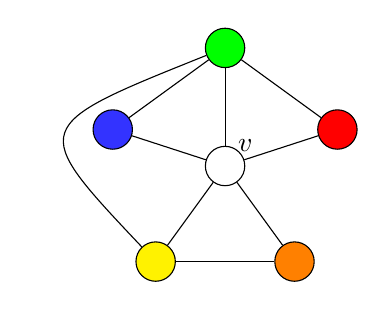
\begin{tikzpicture}[scale=.5,minimum size=5mm,inner sep=0pt]
\foreach \name/\color/\theta in
    {A/red/18,B/green/90,C/blue!80/162,D/yellow/234,E/orange/306}
  \node[circle,draw,fill=\color] (\name) at (\theta:3) {};
\node[circle,draw] (O) at (0,0) {};
\node[above right] at (O) {$v$};
\foreach \name in {A,B,C,D,E}
  \draw (O) -- (\name);
\foreach \i/\j in {A/B,B/C,D/E}
  \draw (\i) -- (\j);
\draw (B) .. controls (-5,1) .. (D);
\end{tikzpicture}
}
\hfill
\rightfigure[c]{
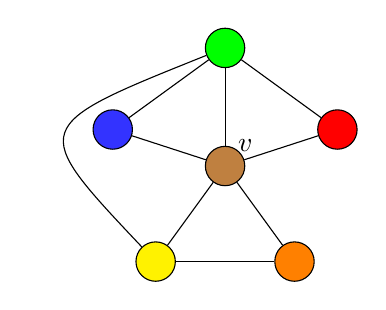
\begin{tikzpicture}[scale=.5,minimum size=5mm,inner sep=0pt]
\foreach \name/\color/\theta in
    {A/red/18,B/green/90,C/blue!80/162,D/yellow/234,E/orange/306}
  \node[circle,draw,fill=\color] (\name) at (\theta:3) {};
\node[circle,draw,fill=brown] (O) at (0,0) {};
\node[above right] at (O) {$v$};
\foreach \name in {A,B,C,D,E}
  \draw (O) -- (\name);
\foreach \i/\j in {A/B,B/C,D/E}
  \draw (\i) -- (\j);
\draw (B) .. controls (-5,1) .. (D);
\end{tikzpicture}
}
\leftcaption{Five colors suffice for coloring the neighbors of $v$}\label{f.five-six-five}
\rightcaption{Color $v$ with the sixth color}\label{f.five-six-six}
\end{figure}

\section{The Five-Color Theorem}\label{s.five-color}

\begin{definition}
Let $G$ be a colored planar graph. A \emph{(Kempe) chain} $G'$ is a maximal, two-colored, connected subgraph of $G$.
\end{definition}\index{Kempe chain}

 
\begin{theorem}\label{thm.fivecolor}
Any planar graph $G$ can be five-colored.
\end{theorem}\index{Five-color theorem}

\begin{proof}
By induction on the number of vertices. If $G$  five vertices or fewer, five colors suffice.
For the inductive step, by Thm.~\ref{thm.degree5} $G$ has a vertex $v$ with degree $5$ or less. Delete $v$ to obtain $G'$. By the induction hypothesis, $G'$ can be five-colored. In $G$, if the degree of $v$ is less than $5$, or if $v_1,\ldots,v_5$, the neighbors of $v$, are colored with four colors or fewer, $v$ can be colored with the fifth color.
Otherwise, $v_1,\ldots,v_5$ are colored with different colors in $G'$ (Fig.~\ref{f.five-color-proof}, top).

\begin{figure}
\begin{center}
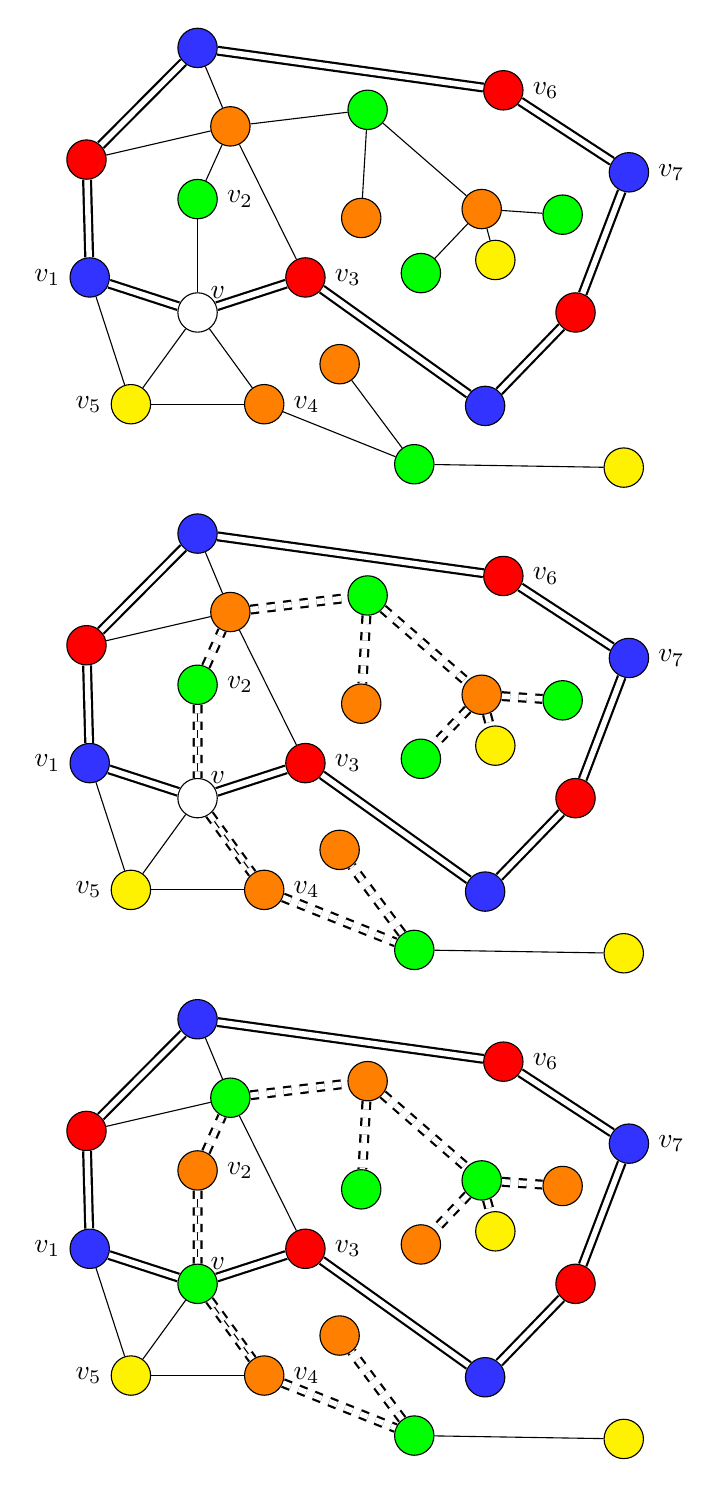
\begin{tikzpicture}[scale=.48,minimum size=5mm,inner sep=0pt]
\foreach \name/\color/\theta in
    {A/red/18,B/green/90,C/blue!80/162,D/yellow/234,E/orange/306}
  \node[circle,draw,fill=\color] (\name) at (\theta:3) {};
\node[circle,draw] (O) at (0,0) {};
\node[above right] at (O) {$v$};

\node[right,xshift=8pt] at (A) {$v_3$};
\node[right,xshift=8pt] at (B) {$v_2$};
\node[left,,xshift=-8pt] at (C) {$v_1$};
\node[left,,xshift=-8pt] at (D) {$v_5$};
\node[right,xshift=8pt] at (E) {$v_4$};

\foreach \name in {A,B,C,D,E}
  \draw (O) -- (\name);
  
\node[circle,draw,fill=red]  (X1) at (126:5) {};
\node[circle,draw,fill=blue!80] (X2) at (90:7)  {};
\node[circle,draw,fill=red]  (X3) at (36:10) {};
\node[right,xshift=8pt] at (X3) {$v_6$};
\node[circle,draw,fill=blue!80] (X4) at (18:12) {};
\node[right,xshift=8pt] at (X4) {$v_7$};
\node[circle,draw,fill=red]  (X5) at (0:10) {};
\node[circle,draw,fill=blue!80] (X6) at (-18:8) {};
\draw[thick,double distance=2pt] (C)  -- (X1);
\draw[thick,double distance=2pt] (X1) -- (X2);
\draw[thick,double distance=2pt] (X2) -- (X3);
\draw[thick,double distance=2pt] (X3) -- (X4);
\draw[thick,double distance=2pt] (X4) -- (X5);
\draw[thick,double distance=2pt] (X5) -- (X6);
\draw[thick,double distance=2pt] (X6) -- (A);
\draw[thick,double distance=2pt] (A) -- (O) -- (C);

\node[circle,draw,fill=orange]  (Y1)  at (80:5) {};
\node[circle,draw,fill=green]   (Y2)  at (50:7)  {};
\node[circle,draw,fill=orange]  (Y3A) at (20:8) {};
\node[circle,draw,fill=orange]  (Y3B) at (30:5) {};
\node[circle,draw,fill=green]   (Y4A) at (10:6) {};
\node[circle,draw,fill=yellow]  (Y4B) at (10:8) {};
\node[circle,draw,fill=green]   (Y4C) at (15:10) {};
\node[circle,draw,fill=green]   (Y5)  at (-35:7) {};
\node[circle,draw,fill=yellow]  (Y6A) at (-20:12) {};
\node[circle,draw,fill=orange]  (Y6B) at (-20:4) {};
\draw (B)  -- (Y1);
\draw (Y1) -- (Y2);
\draw (Y2) -- (Y3A);
\draw (Y2) -- (Y3B);
\draw (Y3A) -- (Y4A);
\draw (Y3A) -- (Y4B);
\draw (Y3A) -- (Y4C);
\draw (E)  -- (Y5);
\draw (Y5) -- (Y6A);
\draw (Y5) -- (Y6B);
\draw (A) -- (Y1);
\draw (X2) -- (Y1);
\draw (X1) -- (Y1);
\draw (D) -- (E);
\draw (D) -- (C);

\begin{scope}[yshift=-12.85cm]
\foreach \name/\color/\theta in
    {A/red/18,B/green/90,C/blue!80/162,D/yellow/234,E/orange/306}
  \node[circle,draw,fill=\color] (\name) at (\theta:3) {};
\node[circle,draw] (O) at (0,0) {};
\node[above right] at (O) {$v$};

\node[right,xshift=8pt] at (A) {$v_3$};
\node[right,xshift=8pt] at (B) {$v_2$};
\node[left,,xshift=-8pt] at (C) {$v_1$};
\node[left,,xshift=-8pt] at (D) {$v_5$};
\node[right,xshift=8pt] at (E) {$v_4$};

\foreach \name in {A,B,C,D,E}
  \draw (O) -- (\name);
  
\node[circle,draw,fill=red]  (X1) at (126:5) {};
\node[circle,draw,fill=blue!80] (X2) at (90:7)  {};
\node[circle,draw,fill=red]  (X3) at (36:10) {};
\node[circle,draw,fill=blue!80] (X4) at (18:12) {};
\node[circle,draw,fill=red]  (X5) at (0:10) {};
\node[circle,draw,fill=blue!80] (X6) at (-18:8) {};

\draw[thick,double distance=2pt] (C)  -- (X1);
\draw[thick,double distance=2pt] (X1) -- (X2);
\draw[thick,double distance=2pt] (X2) -- (X3);
\draw[thick,double distance=2pt] (X3) -- (X4);
\draw[thick,double distance=2pt] (X4) -- (X5);
\draw[thick,double distance=2pt] (X5) -- (X6);
\draw[thick,double distance=2pt] (X6) -- (A);
\draw[thick,double distance=2pt] (A) -- (O) -- (C);

\node[circle,draw,fill=orange]  (Y1)  at (80:5) {};
\node[circle,draw,fill=green]   (Y2)  at (50:7)  {};
\node[circle,draw,fill=orange]  (Y3A) at (20:8) {};
\node[circle,draw,fill=orange]  (Y3B) at (30:5) {};
\node[circle,draw,fill=green]   (Y4A) at (10:6) {};
\node[circle,draw,fill=yellow]   (Y4B) at (10:8) {};
\node[circle,draw,fill=green]   (Y4C) at (15:10) {};
\node[circle,draw,fill=green]   (Y5)  at (-35:7) {};
\node[circle,draw,fill=yellow]  (Y6A) at (-20:12) {};
\node[circle,draw,fill=orange]  (Y6B) at (-20:4) {};
\draw[thick,dashed,double distance=2pt] (B)  -- (O) -- (E);
\draw[thick,dashed,double distance=2pt] (B)  -- (Y1);
\draw[thick,dashed,double distance=2pt] (Y1) -- (Y2);
\draw[thick,dashed,double distance=2pt] (Y2) -- (Y3A);
\draw[thick,dashed,double distance=2pt] (Y2) -- (Y3B);
\draw[thick,dashed,double distance=2pt] (Y3A) -- (Y4A);
\draw[thick,dashed,double distance=2pt] (Y3A) -- (Y4B);
\draw[thick,dashed,double distance=2pt] (Y3A) -- (Y4C);
\draw[thick,dashed,double distance=2pt] (E)  -- (Y5);
\draw[thick,dashed,double distance=2pt] (Y5) -- (Y6B);
\draw (Y5) -- (Y6A);
\draw (A) -- (Y1);
\draw (X2) -- (Y1);
\draw (X1) -- (Y1);
\draw (D) -- (E);
\draw (D) -- (C);
\node[right,xshift=8pt] at (X3) {$v_6$};
\node[right,xshift=8pt] at (X4) {$v_7$};
\end{scope}

\begin{scope}[yshift=-25.7cm]
\foreach \name/\color/\theta in
    {A/red/18,B/orange/90,C/blue!80/162,D/yellow/234,E/orange/306}
  \node[circle,draw,fill=\color] (\name) at (\theta:3) {};
\node[circle,draw,fill=green] (O) at (0,0) {};
\node[above right] at (O) {$v$};

\node[right,xshift=8pt] at (A) {$v_3$};
\node[right,xshift=8pt] at (B) {$v_2$};
\node[left,,xshift=-8pt] at (C) {$v_1$};
\node[left,,xshift=-8pt] at (D) {$v_5$};
\node[right,xshift=8pt] at (E) {$v_4$};

\foreach \name in {A,B,C,D,E}
  \draw (O) -- (\name);
  
\node[circle,draw,fill=red]  (X1) at (126:5) {};
\node[circle,draw,fill=blue!80] (X2) at (90:7)  {};
\node[circle,draw,fill=red]  (X3) at (36:10) {};
\node[circle,draw,fill=blue!80] (X4) at (18:12) {};
\node[circle,draw,fill=red]  (X5) at (0:10) {};
\node[circle,draw,fill=blue!80] (X6) at (-18:8) {};

\draw[thick,double distance=2pt] (C)  -- (X1);
\draw[thick,double distance=2pt] (X1) -- (X2);
\draw[thick,double distance=2pt] (X2) -- (X3);
\draw[thick,double distance=2pt] (X3) -- (X4);
\draw[thick,double distance=2pt] (X4) -- (X5);
\draw[thick,double distance=2pt] (X5) -- (X6);
\draw[thick,double distance=2pt] (X6) -- (A);
\draw[thick,double distance=2pt] (A) -- (O) -- (C);

\node[circle,draw,fill=green]  (Y1)  at (80:5) {};
\node[circle,draw,fill=orange]   (Y2)  at (50:7)  {};
\node[circle,draw,fill=green]  (Y3A) at (20:8) {};
\node[circle,draw,fill=green]  (Y3B) at (30:5) {};
\node[circle,draw,fill=orange]   (Y4A) at (10:6) {};
\node[circle,draw,fill=yellow]   (Y4B) at (10:8) {};
\node[circle,draw,fill=orange]   (Y4C) at (15:10) {};
\node[circle,draw,fill=green]   (Y5)  at (-35:7) {};
\node[circle,draw,fill=yellow]  (Y6A) at (-20:12) {};
\node[circle,draw,fill=orange]  (Y6B) at (-20:4) {};

\draw[thick,dashed,double distance=2pt] (B)  -- (O) -- (E);
\draw[thick,dashed,double distance=2pt] (B)  -- (Y1);
\draw[thick,dashed,double distance=2pt] (Y1) -- (Y2);
\draw[thick,dashed,double distance=2pt] (Y2) -- (Y3A);
\draw[thick,dashed,double distance=2pt] (Y2) -- (Y3B);
\draw[thick,dashed,double distance=2pt] (Y3A) -- (Y4A);
\draw[thick,dashed,double distance=2pt] (Y3A) -- (Y4B);
\draw[thick,dashed,double distance=2pt] (Y3A) -- (Y4C);
\draw[thick,dashed,double distance=2pt] (E)  -- (Y5);
\draw[thick,dashed,double distance=2pt] (Y5) -- (Y6B);


\draw (Y5) -- (Y6A);
\draw (A) -- (Y1);
\draw (X2) -- (Y1);
\draw (X1) -- (Y1);
\draw (D) -- (E);
\draw (D) -- (C);
\node[right,xshift=8pt] at (X3) {$v_6$};
\node[right,xshift=8pt] at (X4) {$v_7$};
\end{scope}
\end{tikzpicture}
\end{center}
\caption{Proof of the five-color theorem}\label{f.five-color-proof}
\end{figure}

\clearpage

Consider vertex $v_1$ which is colored blue and vertex $v_3$ which is colored red. If $v_1,v_3$ are not connected (say if the edge $\overline{v_6v_7}$ did not exist), we can exchange the colors along the path from $v_1$ to $v_6$ and color $v$ blue. Otherwise, consider the blue-red chain which contains $v_1,v_3$. By adding $v$ and the edges $\overline{vv_1},\overline{vv_3}$ we obtain a closed path $P$ (double line) that divides the plane into an ``inside'' region and an ``outside'' region (Fig.~\ref{f.five-color-proof}, middle)

Consider $v_2$ which is colored green and $v_4$ which is colored orange. These vertices \emph{cannot} be contained in a single green-orange chain, because $v_2$ is \emph{inside} $P$ and $v_4$ is \emph{outside} $P$, so any path connecting them must cross $P$, contradicting the assumption that the graph is planar. Therefore, they must be contained in two \emph{unconnected} green-orange chains (double dashed line, in Fig.~\ref{f.five-color-proof}, middle).
Exchange the colors on the chain containing $v_2$ and then $v$ can be colored green to obtain a five-coloring of $G$ (Fig.~\ref{f.five-color-proof}, bottom).
\end{proof}

\begin{advanced}
The statement that a continuous path from the \emph{inside} of of a closed continuous curve $P$ to the \emph{outside} of $P$ must intersect $P$ is the \textbf{Jordan Curve Theorem}. The theorem is intuitively obvious but difficult to prove.
\end{advanced}

\section{Kempe's Incorrect Proof of the Four-Color Theorem}\label{s.kempe}

\begin{theorem}\label{thm.fourcolor}
Any planar graph $G$ can be four-colored.
\end{theorem}\index{Four-color theorem}

\begin{proof}[Incorrect] The base case of the induction and most of the proof is the same as that of the five-color theorem. The new case that must be considered is a vertex $v$ with five neighbors which, by the inductive hypothesis, can be colored with four colors after removing $v$.

In Fig.~\ref{f.five-kempe1} there are two vertices $v_2,v_5$ colored blue. Consider the blue-green chain containing $v_2$ and the blue-yellow chain containing $v_5$. The blue-green chain is contained within the closed path defined by the red-yellow chain containing $v_1,v_3$ (double line) and the blue-yellow chain in contained within the closed path defined by the red-green chain containing $v_1,v_4$ (double dashed line).

Exchange the colors of both the blue-green chain and the blue-yellow chain (Fig.~\ref{f.five-kempe1-exchange}). The result is that the neighbors of $v$ are colored with the three colors red, green and yellow, leaving blue free to color $v$.
\end{proof}

\begin{figure}[ht]
\subfigures
\leftfigure[c]{
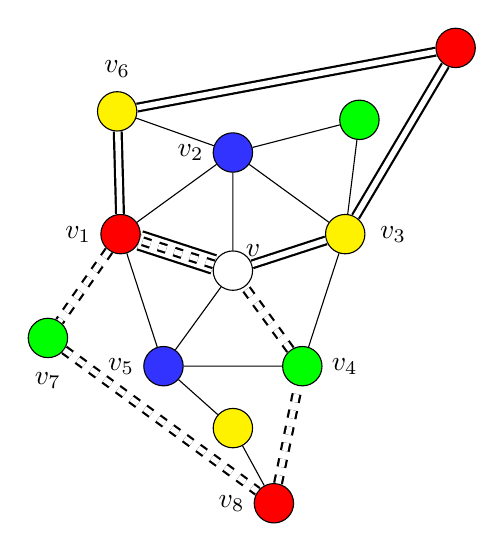
\begin{tikzpicture}[scale=.5,minimum size=5mm,inner sep=0pt]

% Draw center node and adjacent nodes
\foreach \name/\color/\theta in
    {A/yellow/18,B/blue!80/90,C/red/162,D/blue!80/234,E/green/306}
  \node[circle,draw,fill=\color] (\name) at (\theta:3) {};
\node[circle,draw] (O) at (0,0) {};
\node[above right]     at (O) {$v$};

\node[right,xshift=10pt] at (A) {$v_3$};
\node[left,xshift=-8pt]  at (B) {$v_2$};
\node[left,xshift=-8pt]  at (C) {$v_1$};
\node[left,xshift=-8pt]  at (D) {$v_5$};
\node[right,xshift=8pt]  at (E) {$v_4$};

% Draw red-yellow path
\node[circle,draw,fill=yellow]  (X1) at (126:5) {};
\node[circle,draw,fill=red] (X2) at (45:8)  {};

\draw[thick,double distance=2pt] 
  (C) -- (X1) -- (X2) -- (A) -- (O);
\draw[thick,double distance=6pt] (O) -- (C);

% Draw blue-green nodes within red-yellow path
\node[circle,draw,fill=green] (Y1)  at (50:5) {};

% Draw red-green path
\node[circle,draw,fill=green] (Z1)  at (-160:5) {};
\node[circle,draw,fill=red]   (Z2)  at (-80:6)  {};

\draw[thick,dashed,double distance=2pt] 
  (O) -- (C) -- (Z1) -- (Z2) -- (E) -- (O);

% Draw blue-yellow nodes within red-green path
\node[circle,draw,fill=yellow]   (U1)  at (-90:4)  {};

% Connect adjacent nodes not in paths
\draw (X1) -- (B) -- (Y1) -- (A) -- (B) -- 
      (C) -- (D) -- (E) -- (A);
\draw (Z2) -- (U1) -- (D) -- (O) -- (B);
\node[above,yshift=8pt] at (X1) {$v_6$};
\node[below,yshift=-8pt] at (Z1) {$v_7$};
\node[left,xshift=-8pt] at (Z2) {$v_8$};
\end{tikzpicture}
}
\hfill
\rightfigure[c]{
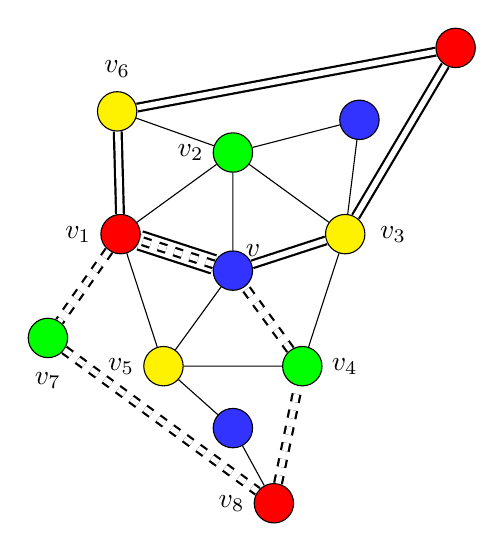
\begin{tikzpicture}[scale=.5,minimum size=5mm,inner sep=0pt]

% Draw center node and adjacent nodes
\foreach \name/\color/\theta in
    {A/yellow/18,B/green/90,C/red/162,D/yellow/234,E/green/306}
  \node[circle,draw,fill=\color] (\name) at (\theta:3) {};
\node[circle,draw,fill=blue!80] (O) at (0,0) {};
\node[above right]     at (O) {$v$};

\node[right,xshift=10pt] at (A) {$v_3$};
\node[left,xshift=-8pt]  at (B) {$v_2$};
\node[left,xshift=-8pt]  at (C) {$v_1$};
\node[left,xshift=-8pt]  at (D) {$v_5$};
\node[right,xshift=8pt]  at (E) {$v_4$};

% Draw red-yellow path
\node[circle,draw,fill=yellow]  (X1) at (126:5) {};
\node[circle,draw,fill=red] (X2) at (45:8)  {};

\draw[thick,double distance=2pt] 
  (C) -- (X1) -- (X2) -- (A) -- (O);
\draw[thick,double distance=6pt] (O) -- (C);

% Draw blue-green nodes within red-yellow path
\node[circle,draw,fill=blue!80] (Y1)  at (50:5) {};

% Draw red-green path
\node[circle,draw,fill=green] (Z1)  at (-160:5) {};
\node[circle,draw,fill=red]   (Z2)  at (-80:6)  {};

\draw[thick,dashed,double distance=2pt] 
  (O) -- (C) -- (Z1) -- (Z2) -- (E) -- (O);

% Draw blue-yellow nodes within red-green path
\node[circle,draw,fill=blue!80]   (U1)  at (-90:4)  {};

% Connect adjacent nodes not in paths
\draw (X1) -- (B) -- (Y1) -- (A) -- (B) -- 
      (C) -- (D) -- (E) -- (A);
\draw (Z2) -- (U1) -- (D) -- (O) -- (B);
\node[above,yshift=8pt] at (X1) {$v_6$};
\node[below,yshift=-8pt] at (Z1) {$v_7$};
\node[left,xshift=-8pt] at (Z2) {$v_8$};
\end{tikzpicture}
}
\leftcaption{Blue-green and blue-yellow Kempe chains}\label{f.five-kempe1}
\rightcaption{Exchange the colors of the two Kempe chains}\label{f.five-kempe1-exchange}
\end{figure}

Heawood noted that the closed paths defined by the red-yellow chain and the red-green chain can share red vertices ($v_1,v_8$ in Fig.~\ref{f.five-kempe2}). When the colors are exchanged in the blue-green and blue-yellow chains, it is possible for blue vertices $v_6,v_7$ to be connected (Fig.~\ref{f.five-kempe2-share}) and the coloring is no longer correct.


\begin{figure}[ht]
\subfigures
\leftfigure[c]{
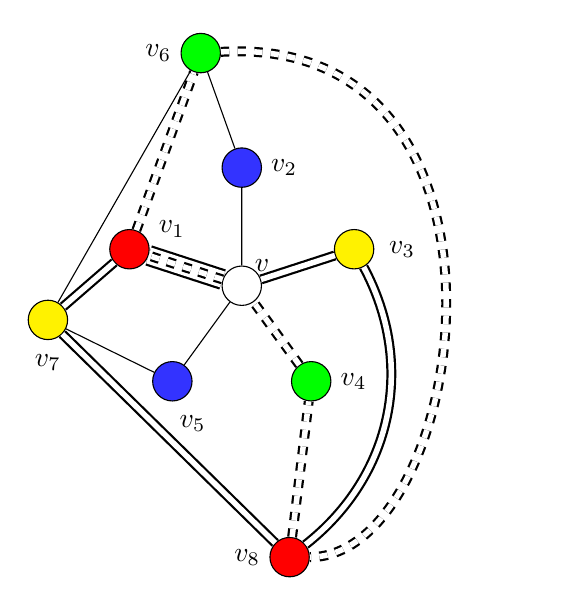
\begin{tikzpicture}[scale=.5,minimum size=5mm,inner sep=0pt]

% Draw center node and adjacent nodes
\foreach \name/\color/\theta in
    {A/yellow/18,B/blue!80/90,C/red/162,D/blue!80/234,E/green/306}
  \node[circle,draw,fill=\color] (\name) at (\theta:3) {};
\node[circle,draw] (O) at (0,0) {};
\node[above right]     at (O) {$v$};

\node[right,xshift=10pt] at (A) {$v_3$};
\node[right,xshift=8pt]  at (B) {$v_2$};
\node[above right,xshift=8pt]  at (C) {$v_1$};
\node[below right,yshift=-8pt] at (D) {$v_5$};
\node[right,xshift=8pt]  at (E) {$v_4$};

% Draw red-yellow path
\node[circle,draw,fill=yellow] (X1) at (-170:5) {};
\node[circle,draw,fill=red]    (X2) at (-80:7)  {};

\draw[thick,double distance=2pt] (A) -- (O);
\draw[thick,double distance=6pt] (O) -- (C);
\draw[thick,double distance=2pt] (C) --(X1) -- (X2);
\draw[thick,double distance=2pt,bend right=40] (X2) to (A);

% Draw red-green path
\node[circle,draw,fill=green] (Y1) at (100:6)  {};

\draw[dashed,thick,double distance=2pt] (O) -- (C) -- (Y1);
\draw[dashed,thick,double distance=2pt] 
  (Y1) .. controls (40:10) and (-50:9) .. (X2);
\draw[dashed,thick,double distance=2pt] (X2) -- (E) -- (O);

% Draw adjacent nodes
\draw (X1) -- (D) -- (O) -- (B) -- (Y1) -- (X1);
\node[left,xshift=-8pt] at (Y1) {$v_6$};
\node[below,yshift=-8pt] at (X1) {$v_7$};
\node[left,xshift=-8pt] at (X2) {$v_8$};
\end{tikzpicture}
}
\hfill
\rightfigure[c]{
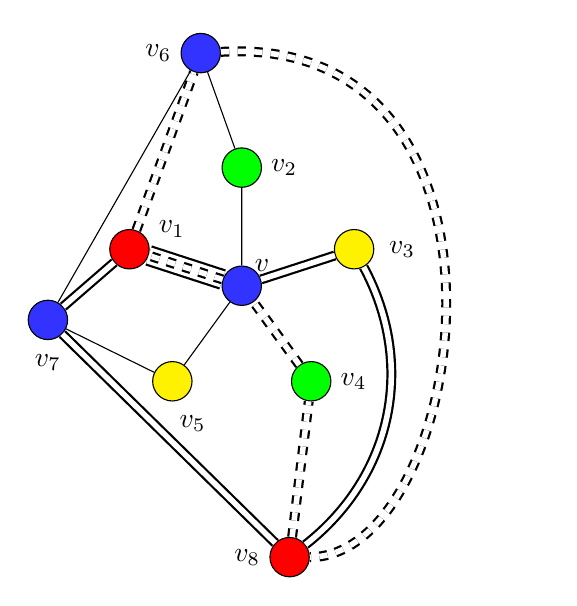
\begin{tikzpicture}[scale=.5,minimum size=5mm,inner sep=0pt]

% Draw center node and adjacent nodes
\foreach \name/\color/\theta in
    {A/yellow/18,B/green/90,C/red/162,D/yellow/234,E/green/306}
  \node[circle,draw,fill=\color] (\name) at (\theta:3) {};
\node[circle,draw,fill=blue!80] (O) at (0,0) {};
\node[above right]     at (O) {$v$};

\node[right,xshift=10pt] at (A) {$v_3$};
\node[right,xshift=8pt]  at (B) {$v_2$};
\node[above right,xshift=8pt]  at (C) {$v_1$};
\node[below right,yshift=-8pt] at (D) {$v_5$};
\node[right,xshift=8pt]  at (E) {$v_4$};

% Draw red-yellow path
\node[circle,draw,fill=blue!80] (X1) at (-170:5) {};
\node[circle,draw,fill=red]  (X2) at (-80:7)  {};

\draw[thick,double distance=2pt] (A) -- (O);
\draw[thick,double distance=6pt] (O) -- (C);
\draw[thick,double distance=2pt] (C) --(X1) -- (X2);
\draw[thick,double distance=2pt,bend right=40] (X2) to (A);

% Draw red-green path
\node[circle,draw,fill=blue!80] (Y1) at (100:6)  {};

\draw[dashed,thick,double distance=2pt] (O) -- (C) -- (Y1);
\draw[dashed,thick,double distance=2pt] 
  (Y1) .. controls (40:10) and (-50:9) .. (X2);
\draw[dashed,thick,double distance=2pt] (X2) -- (E) -- (O);

% Draw adjacent nodes
\draw (X1) -- (D) -- (O) -- (B) -- (Y1) -- (X1);
\node[left,xshift=-8pt] at (Y1) {$v_6$};
\node[below,yshift=-8pt] at (X1) {$v_7$};
\node[left,xshift=-8pt] at (X2) {$v_8$};
\end{tikzpicture}
}
\leftcaption{Red-yellow and red-green chains share red vertices}\label{f.five-kempe2}
\rightcaption{Exchanging colors causes the blue vertices to become connected}\label{f.five-kempe2-share}
\end{figure}

\clearpage

\subsection*{What Is the Surprise?}

The four-color theorem is notorious because it is so easy to state but extremely difficult to prove. Therefore, it is surprising that the proof of the five-color theorem is elementary. The clever part of the proof is Thm.~\ref{thm.degree5} (a planar graph must have a vertex of at most degree $5$), which is a theorem that has nothing to do with coloring. Instead, it results just from counting vertices and edges.

\subsection*{Sources}
On the four-color theorem see \cite{thomas,wiki:four}. The proof of the five-color theorem is based on \cite{thebook,wiki:five}.
\cite{eppstein} presents numerous proofs of Euler's formula. Kempe's incorrect proof of the four-color theorem is described in \cite{sipka}.
